\documentclass[fleqn,11pt]{wlscirep}
\usepackage[utf8]{inputenc}
\usepackage[T1]{fontenc}
\usepackage{eucal}
\usepackage[mathcal]{eucal}

\usepackage{bm}
\newcommand{\ydnote}[1]{\textcolor{red}{#1}}
\title{  Fault detection and diagnosis in CSTR reactor with a hybrid knowledge-machine learning approach}

\author[1,*]{Yong Dou(yd2373)}

\affil[1]{Columbia University, Department of Chemical Engineering ,New York, NY}

\affil[*]{e-mail:yd2373@columbia.edu}
\begin{abstract}
 Continuous stirred-tank reactor(CSTR) is a widely used continous operation reactor model in chemical or pharmaceutical engineering.(The schematic of a typical CSTR is shown in figure 1) CSTR assumes an almost perfect mixed reactor with stable flow input and output. CSTR is feasible with multi-phase reaction with good temperature control, economic cost and unsophisticated system.\cite{fogler2010essentials}  However CSTR sometimes may face the problems to cause fault in the unit operation such as low conversion rate and poor agitation in reactor. In the real industry, it is very important to detect fault in CSTR for safety and efficiency. The aim of this paper is to introduce an AI approach to detect the fault in CSTR. The first part of the paper is to introduce the basic mechanism of CSTR and review some similar approach of fault detection in CSTR and the second is to show the methodology used in the paper; the third of the paper is the results and discussion on fault detection: our machine learning model can predict with accuracy close to 1 and we also build a knowledge based model to detect the fault.
\end{abstract}


\begin{document}

\flushbottom
\maketitle

\thispagestyle{empty}

\noindent \textbf{Key points:}  CSTR, Fault Detection, Knowledge-based System, Machine Learning}

\section{Introduction}
\textbf{Transport process and heat exchange in CSTR:} As shown in the figure 1, CSTR is a dynamics transport process with mass and heat input as well as internal consumption and production via reaction. A normal functional CSTR reactor is usually in a steady state so that the flux in/out of the reactor are the same to keep a constant reaction volume inside the reactor. The mass balance can be represented by(with the assumption of constant density):
\begin{equation}
    v_{inlet}(C_{inlet}-C_{reactor})=V R\left\{k(T_{reactor}),C_{reactor}\right\}
\end{equation}
Where $V_{inlet}$ is the flow rate; $C_{inlet},C_{reactor}$ are the concentration of reactant in the feed flux and reactor separately; $V$ is the volume of reactor;R is the reaction rate as a function of temperature in reactor $T_{reactor}$(reaction constant$k(T)$ depends on temperature) and $C_{reactor}$.  The reaction constant can be expressed as with arrhenius equation 
\begin{equation} 
    k(T_{reactor})=k(T_{inlet})Exp\left[\frac{E}{RT_{inlet}} \frac{T_{reactor}-T_{inlet}}{T_{reactor}}\right]
\end{equation}


If the reaction is a first order reaction, the right part of equation(1) can be simplified as $Vk(T_{reactor})C_{reactor}$. In the steady state,  the output concentration and temperature of CSTR is same the concentration and temperature inside the reactor. Thus, the output of a CSTR is  a function of residence time and rate of reaction. Damköhler number is used to describe this kind of reactions defined as
\begin{equation}
    Da=\frac{reaction rate}{flow}
\end{equation}
 Levenspiel Plot which represent the relationship between  Damköhler number and conversion rate  is often used to help design the volume of reactor\cite{fogler2010essentials}.
\begin{figure}[h]
    \centering
    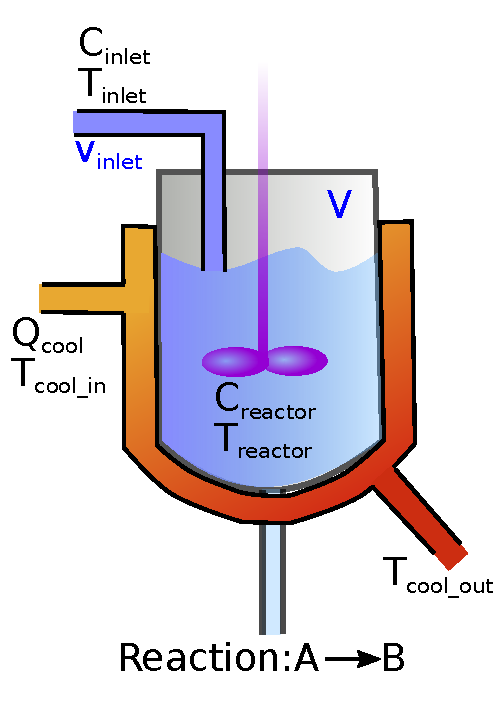
\includegraphics[width=8.5cm]{CSTR.pdf}
    \caption{
    \textbf{Schematic of CSTR } The continuous feed flow with temperature $T_{inlet}$ and reactant concentration $C_{inlet}$ is pumped into reactor. To keep an isothermal reacting environment, a coolant with flux $Q_{cool}$ and temperature $T_{cool_in} $ is used to finish the heat exchange target.Black parameters are known parameters in this paper while some hidden parameters  are shown in blue For the simplicity, no sensors/valves are plotted here.}
    \label{fig:1}
\end{figure}

While some CSTR is operated is in non-isothermal state\cite{bruns1977nonlinear}, CSTR is usually operated in a isotermal state\cite{balakotaiah1981analysis}. If the reaction is exothermic, to keep a constant temperature inside reactor, a coolant(as shown in the figure 1) is required to finish heat transfer target. The heat balance can be expressed as:

\begin{equation} 
    v \rho \mathcal{C}(T_{inlet}-T_{reactor})+V(-\Delta H)R\left\{k(T_{reactor}),C_{reactor}\right\}=(T_{cool\_out}-T_{cool\_in})Q_{cool} \mathcal{C}
\end{equation}
Where $\rho$ is the density of fluid and $\mathcal{C}$ is the heat capacity of fluid; $\delta H$ is the enthalpy of the reaction;$Q_{cool}$ is the flowrate of coolant and $T_{cool\_out}, T_{cool\_in}$ are the inlet and outlet temperature of coolant. In addition to the simple CSTR model above, there has been lots of research on more complex situation such as non-steady state CSTR with dynamics behaviors \cite{balakotaiah1981analysis,schmidt1981dynamic} ,non-isothermal CSTR \cite{hamer1981dynamic} and complex reaction \cite{scott1983reversible,lin1981multiplicity}. I would like to refer audience Professor W. Harmon Ray's elegant series papers  on CSTR \cite{teymour1989dynamic,teymour1992dynamic,teymour1992dynamic2}  to learn more about CSTR system. 

\textbf{CSTR fault detection :} In the real industrial operation, the CSTR is very different from the simple model presented above with the existence of supporting part such as valves, sensors , pipes and feedback system which add lots of measure able/hidden parameters. It is very important to detect the fault and diagnose the reason quickly and efficiently for safety and productivity. However, simply using several differential equations is not enough to describe the complex system. The research on fault detection for CSTR has a very long history in chemical engineering field, which can be dated back 1980s. There are mainly three ways to do the fault detection in CSTR: expert system(knowledge based)such as building hierarchical taxonomy relations with physical/chemical understanding  of CSTR system\cite{chang1990line,terpstra1992real}; machine learning(data driven) such a artificial neural network\cite{hoskins1991fault}; and hybrid model which combined previous two method together\cite{ozyurt1996hybrid,zhang1996process}.  These papers back to more than 10 years ago are limited to the computation ability and the amount of clear labeled date. With the advent of hardware and computation tools recently, the machine learning approach can be more efficient by incorporating some basic knowledge on CSTR system. And I am going to show this approach in the following content.

\section{Methodology}
\begin{figure}[h]
    \centering
    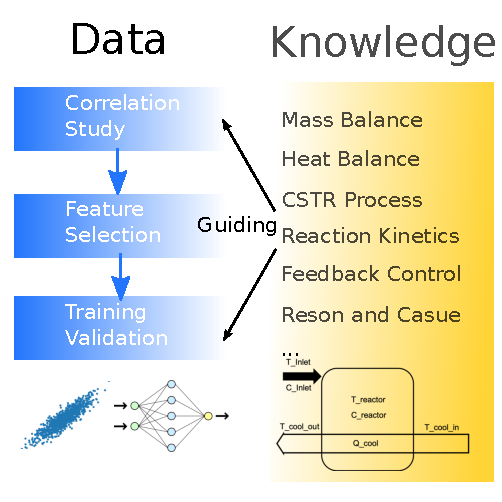
\includegraphics[width=8.5cm]{method.pdf}
    \caption{
    \textbf{Methodology Schematics } The knowledge of CSTR such as mass and heat balance, reaction kinetics are used to check and guide the machine learning process for the labeled date with different fault}
    \label{fig:1}
\end{figure}
To finish a fault detection job, there are 3 steps:1. Realize the existence of fault in CSTR. 2. classify what kind of fault in the system 3. diagnose the real physical/chemical cause for the fault(such as internal or external fault , where is the fault). The data we studied in this paper have already be labeled with 5 different kind of fault as well as the normal steady state. The data have 7 measurable parameters (black parameters in figure 1) which we can use to help detect the fault. However, there are some very important hidden parameters such as feed flow rate and volume of reactor  are not in our date. Because of the lack of measurement of these key parameters, it is not easy to build a full knowledgeable model. Also, because some measurable parameters have physical meaning connection, it is very costly to study pure data(may also cause spurious inferences). In this paper, a hybrid method is used as shown in the figure 2 that the knowledge of CSTR  system is used to check the reasonable of machine learning process. \textbf{First} we check the correlation of the measurable data in the normal operated condition. We use our knowledge of CSTR to understand the correlation of these data. \textbf{Second}  we use feature selection method to select the key features in the classification process and then use our knowledge of CSTR to check the reasonable of the selected feature. We apply the the support vector classification (SVC) to do the feature selection process process because (1)SVC usually has high efficiency with regards to memory (2) the problems happens CSTR usually have very clear margin of separation between classes(such as some parameter is high or low) from our knowledge (3)the data is high dimension with enough data points (4)the measurement in chemical plant is usually accurate with less noise. \textbf{Third} with the selected data, we trained a neural network to do the classification. We add two hidden layers(each have 10 nodes with "relu" as the activation function) to train the neural network.The final layer connected to the final class is activated with "softmax" because this is a classification problem. Moreover, we also used other methods such as K-neartest neighbour and  decision trees to train the data as  a comparison with neural network It seems that all of them works very well.
\textbf{Finally}, we also discuss a little how to built model-based strategy to detect the fault


\section{Results and Discussion.}
\textbf{correlation study of measurable variables in normal data}

According to the equation(4) we can use the data $ Q_{cool}, T_{cool\_in},T_{cool\_out}$ to calculate the heat exchange amount as $heat =Q_{cool}\times( T_{cool\_out}-T_{cool\_out})$, as the eighth feature in the  data. The correlation plot of normal state is shown in the figure 3 as a  pairwise relationship plot for all the eighth variables with r value is the correlation(positive mean means the slop is positive ). It is very clear there several variables are strong correlated while some  variables seems have no relations.We are going to discuss this correlations in the following content.
\begin{figure}[h]
    \centering
    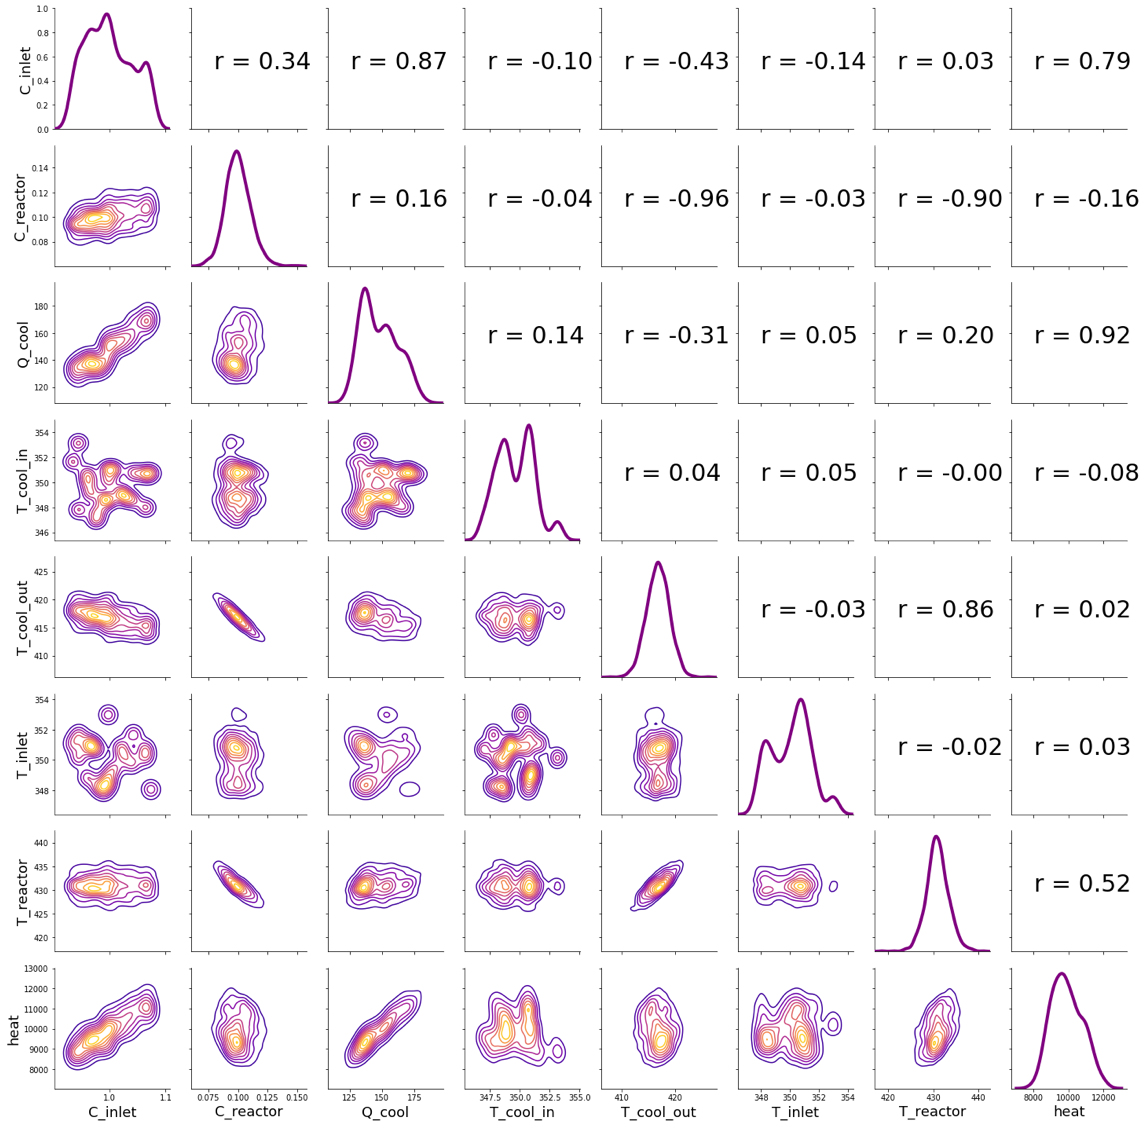
\includegraphics[width=13cm]{figure3.png}
    \caption{
    \textbf{Correlation of different variables in the data labeled as normal  } Kernel density estimation (KDE) is used to show the distribution of each variables in the diagonal. The lower section of plot visualize the  relations between each pair of variables while the upper section shows the  value of correlation. Large absolute value of  correlation indicates strong correlation and   small absolute value of  correlation indicates weak correlation.}
    \label{fig:1}
\end{figure}
\begin{itemize}
     \item {$C_{reactor} ,T_{cool\_out}, r=-0.96$,$C_{reactor} ,T_{reactor},r=-0.9$ ,  $T_{reactor} T_{cool\_out},r=0.86$. These three parameters have the highest correlation. From the mechanism of CSTR we know that, the low concentration in reactor means a high reaction rate happening, which will generate more heat and increase the temperature$T_{reactor}$ in reactor and will lift the output temperature of coolant output$T_{cool\_out}$. We can have the possible relation that  $C_{reactor} \rightarrow T_{reactor} \rightarrow T_{cool\_out} $ } 
      \item {$C_{inlet} ,Q_{cool}, r=0.87$,Increase the feed concentration will increase the temperature of reactor which needs more coolant flux. This high correlation indicate there is some feedback design between the $C_{inlet}$  and $ Q_{cool}$. Also $Q_{cool}$ has  no obvious relations with concentration/temperature in reactor or feed temperature, so we can assume there is not feedback directly between coolant flux and other part in the CSTR system. Now we have another relation that
      $C_{inlet} \rightarrow Q_{cool}$ } 
        \item {$T_{cool\_in} ,T_{inlet}$, These two variables have very small correlations to any variables, which indicate these two are independent variables. This assumption makes lots of sense because these two variables are the outside input into CSTR system(if there is no feedback system connected to them) $T_{cool\_in} ,T_{inlet}$ are both not influenced by the change in system } 
\end{itemize}
Now based on our knowledge of CSTR and the correlation from data, we have a better view of the relations among these data. Fault usually happens from the independent variables (such as$T_{cool\_in} ,T_{inlet}, C_{inlet}$, we use these as our possible candidate for importance feature for training). The problems in dependent variables can usually traced back to these independent variable . 

\textbf{Feature selection}
\begin{figure}[h]
    \centering
    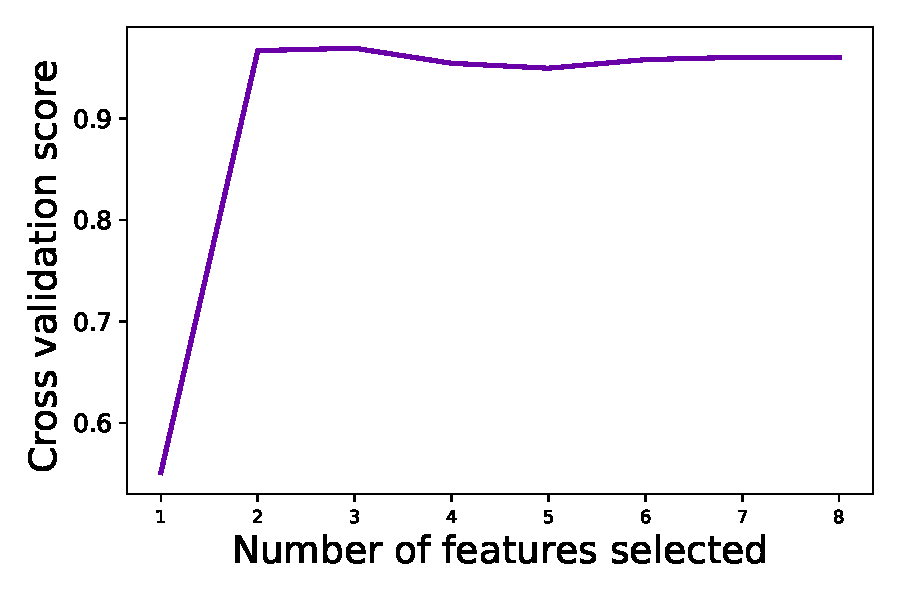
\includegraphics[width=8.5cm]{figure4.pdf}
    \caption{
    \textbf{Feature selection} The ranking of importance of the feature is(from more important to less important): $C_{inlet}, T_{inlet}, Q_{cool}, C_{reactor}, T_{cool\_in}, heat, T_{cool_out}, T_{reactor}$. The cross-validated test score with different number and combination of  features in the system. High test score corresponds to better training results. }
    \label{fig:1}
\end{figure}

 As discussed in the methodology part, we use statistical method to do the feature selection or dimensionality reduction on my data sample. Recursive feature elimination(RFE) can also help us to determine the number of necessary  features to do the training process  
 The ranking of importance of each feature and the RFE plot is shown in the figure 4. Fro, the figure 4, we can see that after we select the two highest ranking features($C_{inlet}, T_{inlet}$), the score is already high enough very close to 1. Adding more features into model don't give better result with a flat platform on score instead. More importantly, the ranking of the importance of features is agree with our knowledge based model  that independent variables($C_{inlet}, T_{inlet},C_{reactor} $) have high score. $C_{inlet}, T_{inlet}$ are the inlet of  system to bring heat and mass into a steady state CSTR reactor, which are physically reasonable to have big possibilities of fault and introducing chaos. The relative low score of independent variables $T_{cool\_in}$ means the fault doesn't come with coolant temperature, which is also physically reasonable due to the less importance of this feature in the CSTR system.Based on the combination of  pure data analysis  and CSTR knowledge, the feature selection has the results of using ($C_{inlet}, T_{inlet}$) as key variables to train the data.
\begin{figure}[h]
    \centering
    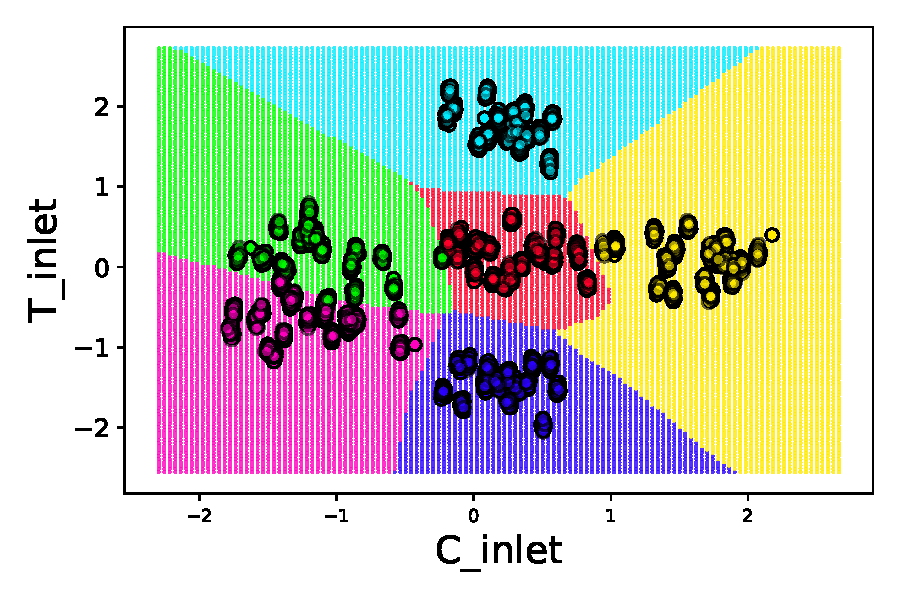
\includegraphics[width=8.5cm]{figure5.pdf}
    \caption{
    \textbf{Training results of neural network} The back ground is the phase plot(or predicted classification results) gained from the neural network. The points plotted are real labeled. The test validation result is 0.9938.  Red : normal; Yellow: fault 1; Green: fault 2; Light blue: fault 3;  Blue: fault 4; Pink:fault 5 }
    \label{fig:1}
\end{figure}
\begin{figure}[h]
    \centering
    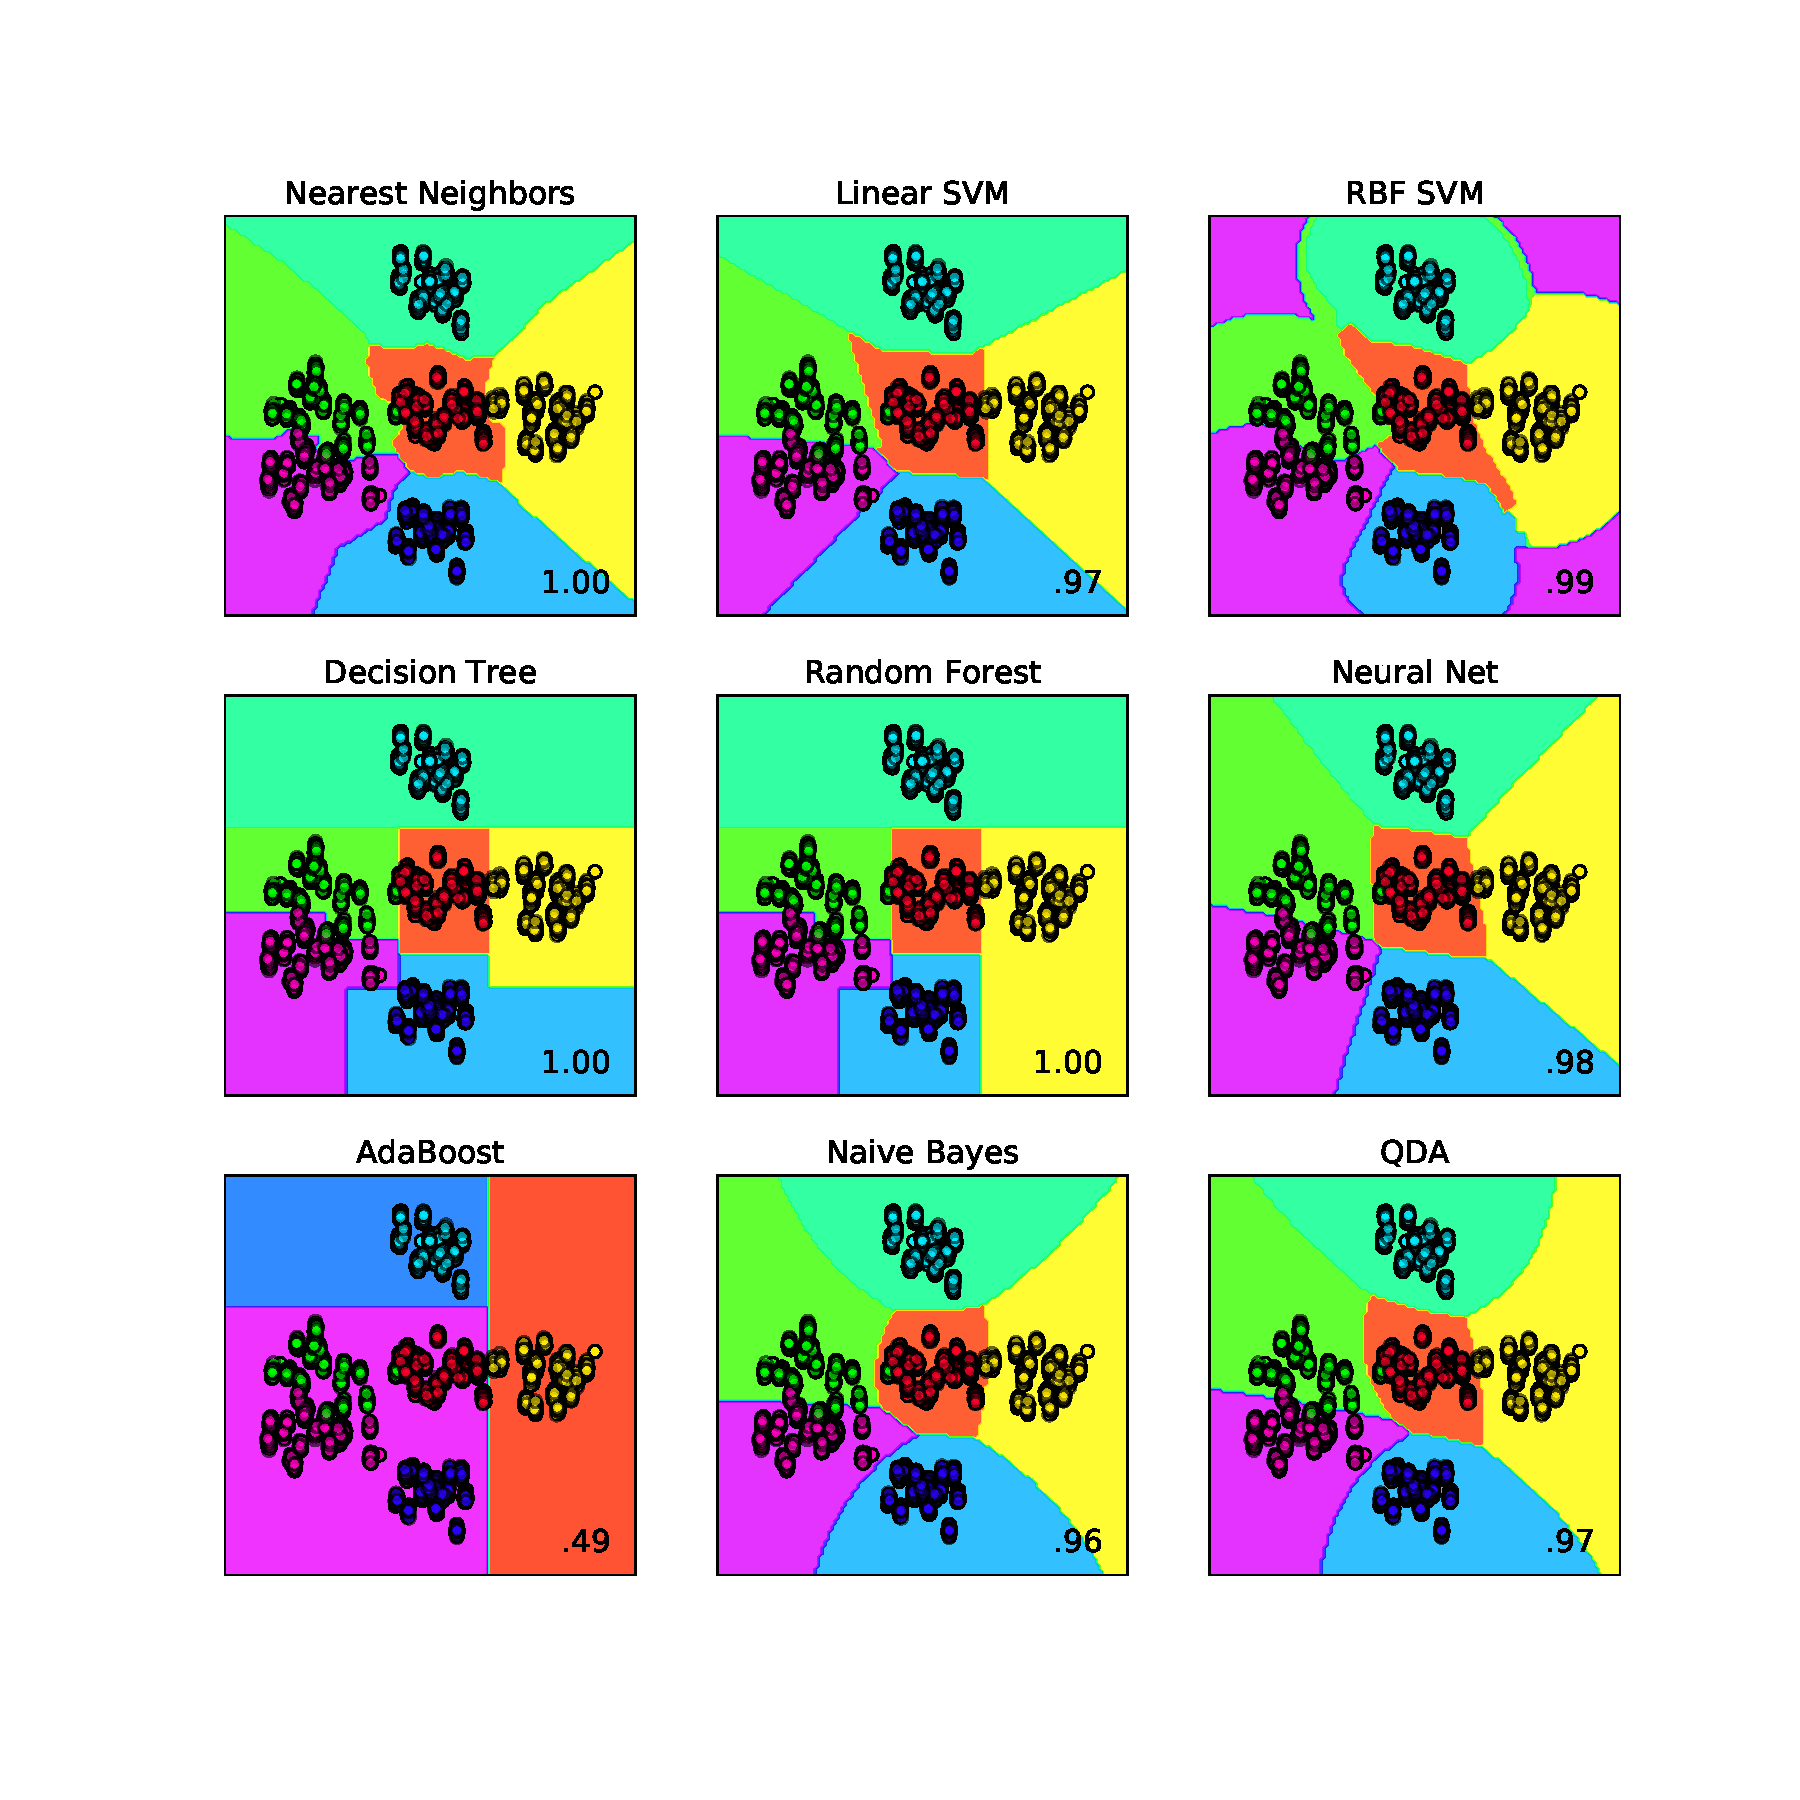
\includegraphics[width=12cm]{figure6.pdf}
    \caption{
    \textbf{Training results of other classification method} The methods of classification are labeled at the title in each subplot. The validation scores are shown at the bottom right at each subplot.  Red : normal; Yellow: fault 1; Green: fault 2; Light blue: fault 3;  Blue: fault 4; Pink:fault 5 }
    \label{fig:1}
\end{figure}
\textbf{Training and validation}

As introduced in the methodology part,two hidden layers are used in the neural network training.Also the raw data are normalized for better training performance.  Stochastic gradient descent is used to optimize the weights in each node and layer.We separated data as training data and test data in the ratio of 80/20.  As a classification problem, categorical$\_$crossentropy is used as the loss function. The training process is operated with 20 epochs and a batch size of 64. The training  result is shown in the figure 5 with an validation accuracy about \textbf{0.9938}. As we can see from the figure 5, the  training result is very good that classify the date into the right fault number. As a comparison, we also applied 9 different other method(as shown in the figure 6). Most of classification methods works very well with an validation accuracy close to 1. Adaboots and supporting vector machine with RBF kernel have unsatisfied results, which could be improved by tuning the parameter in the model carefully(which is not the focus of this paper). Generally, the training process works very well with most  methods and can give very good prediction with a very high accuracy and less over-fitting.


\textbf{Detection and Diagnose }
\begin{figure}[h]
    \centering
    
\includegraphics[width=12cm]{figure7.png}
    \caption{
    \textbf{Diagnose  of the system} The table describes the the direct cause( from the machine learning)of the fault and the system behaviors along the fault( from CSTR knowledge.  }
    \label{fig:1}
\end{figure}

Based on the training results, we summarize the fault type and their possible physical cause in the figure 7. Each fault will lead to series problems in the CSTR system. The real physical cause is complex , which can be the failure of some valves, sensors or pipes, the cause listed in the figures 7 is more like directed cause from key features in data-set.In some extent, this figure(figure 7) can be used as a model to work together with the machine learning results for fault detection. In the future operation, we can online monitor the system and map the measurements into its operation category (such as normal, fault1, fault 2). At the same time we can compare the classification results with the knowledge shown in figure 7 to double check the accuracy of  fault detection. For example , for a type 1 fault in the future operation, we first measure the necessary features and classify it into the fault 1. Then we check whether $C_inlet$ and $Q_cool$ increase or not to double check the classification result from machine learning.
\section{Outlook and Conclusion}
 In this paper, we only discuss 5 type of fault and in the real industry, there will be more fault type. In  addition to detect the fault, we also need to know where is the origin of the fault and the following solution to correct the fault. Before close this paper, I have several outlook and recommendations for the fault detection and diagnose in CSTR with AI approach.
\begin{itemize}
    \item \textbf{Measurement} The high quality  and large amount of data are very essential in the machine learning approach. Although in this paper, we use only 7 variable measurement(after feature selection, it is only 2 feed temperature and concentration , which can be measured with thermometer and some indicator for concentration such as conductivity or  viscosity). For the quality, we need better measurement equipment to acquire the noise free data such as better flow meter, thermo meter, or advanced optical instrument . For the quantity part, we need measure more key features with more data points such as flow rate of feed, volume of reactor. For example, with recent development of image recognition of deep learning, some measurements can be done with high frame rate webcam imaging system. These measurement can help to both train better machine process and built knowledge based system. 
     \item \textbf{Control system} Control system is important to correct the fault. We need to have the knob which can directly or indirectly control the physical variables in the system such as heater/cooler to change the temperature, valve to change the flow rate or concentration. The control systems should also be sensitive and accurate so that they don't introduce new problems.
     \item \textbf{Feedback and AI system} the least but not last is the feedback system and AI system. The feedback system should take reaction from the results by AI system to make CSTR in a stable state. The system we studied in this paper seems only have one feedback system between the coolant flux and feed concentration. A Feedback and AI system for real industry should have lot more feedback loop between pairs of variables.  
\end{itemize}
As a short summary, this paper develop a hybrid AI model with both knowledge and data to detect the fault in CSTR. The model detects the key features of the fault as feed's concentration and temperature. The model has a very high prediction accuracy to the fault detection, which demonstrate the possible application of AI tech in CSTR fault system.

\bibliography{sample}


\end{document}




BY PCA, some physics meaning will be dropped 